%==============================================
%      CHAPTER
%==============================================
\chapter{Discussion}\label{chapter:discussion}

The overall \gls{cv} matrices (see Tables~\ref{table:overall-cv-quad-semi}~to~\ref{table:overall-cv-rigid}) provide useful guidance and insight into which \glspl{vdp} are the most influential in terms of each of the \gls{pbs} performance measures. If a proposed design of a vehicle combination fails a \gls{pbs} assessment, then the columns for the failed \gls{pbs} measures in Tables~\ref{table:overall-cv-quad-semi}~to~\ref{table:overall-cv-rigid} illustrate the \glspl{vdp} which will have the most significant effect in correcting the vehicle performance. Furthermore, when sourcing input data for an assessment, the tables highlight the important \glspl{vdp} which need to be accurately determined i.e. \gls{pbs} assessments should ensure that \glspl{vdp} which significantly affect the \gls{pbs} assessment are accurate and those that don't affect the \gls{pbs} assessment can justifiably use generic approximate data.

Experience has shown that once a vehicle design has been submitted for a \gls{pbs} assessment, there is often little scope to redesign the entire combination since it is either already built or orders for some parts have already been placed. To aid in these situations, separate \gls{cv} matrices were developed for the inertial, geometric, suspension and tyre parameters in isolation with the intention of providing insight into \gls{vdp} influence within each of these categories independent of all other \glspl{vdp}. These matrices can be found in Sections~\ref{section:cv-geometrical}~to~\ref{section:cv-tyre} in Appendix~\ref{appendix:complete-cv-matrix}. These additional matrices are useful in interpreting the overall \gls{cv} matrix. Differences in the relative effect of certain \glspl{vdp} between combinations may be due to other \glspl{vdp} influencing the combination to a greater or lesser extent.

In the sections that follow, insights into the relative influence of heavy vehicle \glspl{vdp} gained from the \gls{cv} matrices are discussed for the most influential \glspl{vdp}. The \glspl{vdp} with a negligible relative influence for all combinations are then listed for quick reference of which \glspl{vdp} could be safely estimated. Finally, limitations of the methodology used in this study are discussed.

%==============================================
%      SECTION
%==============================================
\section{Relative Influence of Heavy Vehicle Design Parameters}\label{section:discussion-relative-influence-of-heavy-vehicle-design-parameters}

Considering the overall \gls{cv} matrices (see Tables~\ref{table:overall-cv-quad-semi}~to~\ref{table:overall-cv-rigid}), the majority of the inertial and geometrical \glspl{vdp} have a significant relative influence on each of the baseline vehicles. With the exception of the moment of inertia, these parameters can easily be determined from a detailed \gls{ga} drawing of a vehicle combination.

A larger proportion of suspension and tyre \glspl{vdp} have a negligible relative influence on vehicle performance relative to the inertial and geometrical \glspl{vdp}. This is important since suspension and tyre details are often difficult to acquire from \glspl{oem}. \glspl{vdp} with negligible relative influence can be conservatively estimated and represent vehicle performance as discussed further in Section~\ref{section:vdps-with-negligible-influence-on-overall-performance}.

%      SUBSECTION
%----------------------------------------------
\subsection{Geometrical and Inertial VDPs}\label{section:geometrical-and-inertial-vdps}

The \textbf{wheelbase} has a significant relative influence on high-speed and low-speed standards for all baseline combinations. It has a high to negligible relative influence on the longitudinal standards depending on the baseline vehicle.

The prime mover wheelbase has a medium to high relative influence on \gls{graa}, \gls{hsto}, \gls{lssp}, \gls{fs} and \gls{stfd} for all baseline vehicles. It has a high influence on the \gls{ts} for the rigid drawbar baseline since the critical reference point for \gls{ts} in its baseline configuration is the rear of the rigid truck superstructure whereas for the other baselines the critical point is at the rear of the rearmost trailer.

The trailer wheelbase (predominantly the follower trailer for the tridem interlink) has the maximum influence on \gls{lssp} for all combinations and has a medium to high influence on \gls{ts}. It has a medium to high influence on the high-speed standards \gls{ydc}, \gls{ra} and \gls{hsto} with the exception of it having a low influence on \gls{ra} for the tridem interlink combination.

The rigid drawbar combination dolly wheelbase has a medium influence on the \gls{lssp} with negligible influence on all other performance measures.

The \textbf{moment of inertia} has a relatively low influence with the exception of the trailer payload pitch and yaw moment of inertia (\gls{iyy}/\gls{izz}) which has a medium to high influence on the \gls{hsto} and \gls{ydc} performance of the quad semi-trailer and tridem interlink (predominantly for the follower trailer) combinations. 

The pitch and yaw moment of inertia (\gls{iyy}/\gls{izz}) has a low influence on the rigid combination and instead the prime mover payload roll inertia (\gls{ixx}) has a medium influence on \gls{hsto} and \gls{ra}. This highlights that the sensitivity of a combination to the inertial properties is dependent on the mechanics of the articulation points. The results suggest that a combination with roll-coupled articulation points will be affected to a higher degree by a change in pitch and yaw inertia compared to a unit with non roll-coupled articulation points.

The moment of inertia \glspl{vdp} were varied within a large range since they are rarely supplied for \gls{pbs} assessments, vary significantly for different payloads and vehicle configurations, and often need to be estimated using simplified geometries. For a specific commodity and vehicle configuration, these estimations of moments of inertia would differ from the actual inertias by far less than the variation considered in this study. The relatively low influence of the majority of the moments of inertia \glspl{vdp} and the large ranges used for the moments of inertia in this study suggest that using simplified geometries to estimate the moments of inertia is an appropriate approach.

The \textbf{reference point height} has a high influence on the \gls{tasp} of the baseline combinations. The \gls{tasp} manoeuvre involves the combination travelling along a straight path along an uneven surface with an average cross fall of not less than 3\% with the average crossfall standard deviation exceeding 1\% \cite{NationalTransportCommission2008}. The \gls{tasp} performance is measured as the 99\textsuperscript{th} percentile of the swept width between the path of the outer most left and outermost right reference points. The crossfall along with disturbances along the travelled path result in the vehicle rolling and offtracking in the direction of the crossfall during the manoeuvre. The roll motion of vehicle units causes the path scribed in the ground to be projected further in the direction of the roll motion. 

A differential height between the outermost reference points either increases or decreases the measured \gls{tasp} as shown in Figure~\ref{figure:influence-of-reference-point-height-on-tasp}. A worst case \gls{tasp} is measured when the outermost left reference point (point 2 in Figure~\ref{figure:influence-of-reference-point-height-on-tasp}) is low to the ground with the outermost right reference point (point 3 in Figure~\ref{figure:influence-of-reference-point-height-on-tasp}) located at the top of the vehicle structure. The high relative influence of the reference point height on the measured \gls{tasp} highlights a potential for discrepancies in measured \gls{tasp} performance between various assessors depending on the height selected for each reference point. For example, one may ignore a buckle located at the top of a vehicle structure since it is ancillary equipment while another may consider it, resulting in a higher reference point height and higher measured \gls{tasp}.

According to the NTC rules, if multiple points exist at the outermost points, the lowest of that should be chosen. With this definition, if the trailer structure of a combination such as a side tipper was uniform in width rather than having the widest point at the top of the bin, the measured \gls{tasp} performance would be improved even though physically it takes up the same amount of road width. It is suggested that a standard height be determined for reference points to avoid discrepancies in the measurement of the \gls{tasp} performance. In practice this may be difficult for real world tests since a mounting point may not be available, however it is trivial to set a reference point height in a simulation package. 

%----------------------------------------------
%      FIGURE
%----------------------------------------------
\begin{figure}[H]
	\centering
	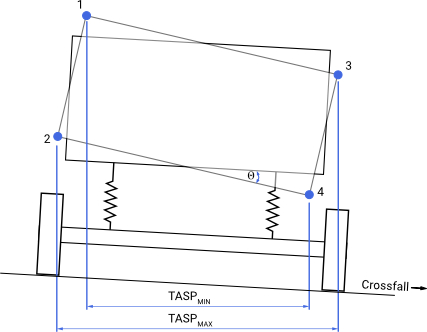
\includegraphics[width=0.7\textwidth]{fig/tasp_reference-point-height-influence}
	\caption{Influence of the reference point height on TASP performance}
	\label{figure:influence-of-reference-point-height-on-tasp}
\end{figure}
%----------------------------------------------
%      FIGURE
%----------------------------------------------

The \textbf{longitudinal standards} consisting of the \gls{sta}, \gls{graa}, \gls{grab} and \gls{acc} performance measures are highly influenced by the payload mass for the tridem interlink and rigid drawbar combination. For the quad semi-trailer, the trailer wheelbase is the most important variable for \gls{sta} and \gls{graa}.

When a heavy vehicle has a sufficiently powered engine, such as in the case of the three baseline combinations, the \gls{sta} and \gls{graa} are dependent on the traction force available at the drive tyres which is a function of the drive axle load when the coefficient of friction is kept constant (the NTC rules state a coefficient of friction of 0.8 should be used for the test road surfaces \cite{NationalTransportCommission2008}). Thus, the \gls{vdp} that has the most relative influence on the vehicle performance would be the one that provides the largest variation on the drive axle load.

The range within which the quad semi-trailer wheelbase was varied led to the wheelbase approaching the combined trailer and payload sprung mass centre of gravity location. At this point, most of the combined sprung mass was supported by the trailer axle group with little load transfer to the prime mover through the 5th wheel hitch. As discussed in Section \ref{section:pr-wheelbase} the legal axle load limits were not considered in determining the range of viable wheelbases as this would limit the allowable wheelbase range for the baseline vehicles and insight would be lost into the effect of changing the wheelbase for combinations that are volume rather than payload limited. For vehicle combinations that are payload limited, the wheelbase will have a smaller range of variation when considering legal axle load limits resulting in a reduced influence.

The \gls{acc} and \gls{graa} tests are performed on a road with a 0\degree{} to 1\degree{} grade respectively and as a result there is always sufficient traction at the drive axle tyres. The \gls{acc} and \gls{graa} performance is therefore limited by the engine power and gross combination mass. The \gls{vdp} providing the most variation in \gls{gcm} becomes the most influential and for all combinations this is the trailer payload. The tridem interlink is equally affected by both trailer payloads since they are identical in mass and were varied within the same range.

The study considered the payload to go from the unladen condition to the maximum laden condition since it is realistic for a combination to operate within that range. In practice, a combination would be optimised for a maximum payload and the payload would have a small envelope of variation. In this case, adjustments to the prime mover engine (which was beyond the scope of this study) and/or geometrical properties which result in a change in drive axle load would provide a larger relative influence.

The \textbf{longitudinal CG location (\gls{cgx})} of the payload has a larger relative influence than those of the prime mover and trailer chassis. The prime mover and trailer chassis \gls{cgx} locations were varied within a larger range (20\% and 30\% respectively) relative to the payload (between 9\% and 13\% depending on baseline combination). However, since the mass of the payload is significantly higher than the chassis in all cases, a change in the payload \gls{cgx} has a higher influence.

The \textbf{lateral CG location (\gls{cgy})} of the payloads (the prime mover and trailer chassis to a much lesser extent) have a medium to high relative influence on the high-speed performance of the combinations, in particular the \gls{srt} and the \gls{srtrrcu}. Therefore it is important to ensure that the \gls{cgy} location is accurately modelled (for payloads in particular) and emphasises that a shift in payload due to poor strapping will have a significant effect on the rollover stability of a vehicle combination. A shift in the \gls{cgy} location in the same direction as the roll motion of the sprung mass will amplify the roll. The additional roll motion will cause the rear reference points to be projected further outward affecting the \gls{tasp} (as discussed above) as well as the \gls{ts} performance of the vehicle.

The \textbf{vertical CG location (\gls{cgz})} of the payload has a high influence on the \gls{srt} and the \gls{srtrrcu} performance for all combinations. This is explained by the simple first-order estimate of \gls{srt} from Gillespie \cite{Gillespie1992} shown in Equation~\ref{eqn:first-order-srt-gillespie} which ignores the effects of deflection in the suspension. The \gls{cgz} has a direct and higher impact on the first-order estimate of \gls{srt} than axle track which is confirmed in the \gls{cv} matrices as the axle track (discussed below) has only a medium influence on \gls{srt} performance.

%----------------------------------------------
%      EQUATION
%----------------------------------------------
\begin{align}
	\label{eqn:first-order-srt-gillespie}
	SRT = \frac{t}{2h}
\end{align}

Where 

$t$ = Vehicle track width (mm)

$h$ = Vertical centre of gravity of the total vehicle mass (mm)

%----------------------------------------------
%      EQUATION
%----------------------------------------------

%      SUBSECTION
%----------------------------------------------
\subsection{Suspension and Tyre VDPs}\label{section:disc-relative-influence-suspension-tyre}

The \textbf{suspension and tyre \glspl{vdp}} have a low to negligible influence on the low-speed standards except for the steer axle track which has a relatively high impact on the \gls{fs} performance. The \gls{fs} performance of a combination is measured as the swing out of the front of the cab relative to the steer axle path inscribed on the ground at the outer edge of the steer tyre around a 90\degree{} turn \cite{NationalTransportCommission2008}. Considering that the cab dimensions remain constant, a wider steer axle track reduces the \gls{fs} and a narrower track width increases the \gls{fs} of the combination. Within the range of evaluated steer axle track widths, the axle track has a high influence on the \gls{fs} performance for all combinations.

The \textbf{trailer axle track} for the tridem interlink and rigid combination have a medium influence on the \gls{srt} performance while it has a low influence on the \gls{srt} performance of the quad semi-trailer. The minimum axle track for the trailer axle with 445/65 R22.5 single tyres is close to the maximum for the other baseline combinations. The roll stiffness of the quad semi-trailer is therefore still high even at the minimum axle track and therefore other parameters have a larger effect on the \gls{srt} performance of the vehicle, diminishing the relative effect of the trailer axle track for this combination.

The \textbf{drive axle auxiliary roll stiffness} has a larger relative influence on the performance of the rigid drawbar combination. The rigid drawbar combination has a pintle hitch which is a non roll-coupled hitch. Thus, roll effects are not transferred between the trailer and rigid unit. The rigid prime mover acts as a single unit and the dolly along with the trailer act as the rearward roll coupled unit which are connected with a roll-coupled hitch (5th wheel) allowing transfer of roll moments between the dolly and trailer. Decreasing the auxiliary roll stiffness on the rigid prime mover degrades the overall roll stiffness of the prime mover to a larger degree than the other combinations since it is not assisted by the roll stiffness of the trailers. The amplified roll experienced by the rigid prime mover results in degraded high-speed performance. This suggests that compared to a combination with roll-coupled hitch points, a combination with non roll-coupled hitch points will be affected by a greater degree when the auxiliary roll stiffness is adjusted on a single vehicle unit.

The \textbf{trailer axle auxiliary roll stiffness} has a medium relative influence on \gls{tasp} and low to negligible influence on all other performance measures for the quad semi-trailer. In the case of the tridem interlink and rigid combination, trailer axle auxiliary roll stiffness has a medium to high influence on \gls{srt}, \gls{ydc}, \gls{ra} and \gls{hsto} and the maximum effect on \gls{tasp}.

The greater influence of trailer axle auxiliary roll stiffness on the \gls{ra} of the tridem interlink (maximum influence) and rigid drawbar combination (high influence) relative to the quad semi-trailer (negligible influence) can be explained when considering the overall roll stiffness. The wider axle track and increased number of axles on the trailer unit of the quad semi-trailer results in the combination having a high overall roll stiffness even with a low auxiliary roll stiffness. The tridem interlink has the narrowest axle track which exacerbates the effect of decreasing the trailer auxiliary roll stiffness and results in the trailer axle auxiliary roll stiffness having the maximum influence on \gls{ra} for this combination.

The baseline vehicles have reference points at the top of the trailer structure which assumes that the outermost point on the right of the vehicle is at the top of the trailer structure. This is typical of tautliners with buckles and side-tippers with the widest point at the top of the bin. The outermost left reference point is located near to the ground on the bumper of the prime mover. If the rear reference points were lower to the ground (at the base of the trailer deck for example), the height differential between the left and right outer reference points would be decreased. This would decrease how far outwards the reference points are extended from each other for a given amount of roll (see Figure~\ref{figure:influence-of-reference-point-height-on-tasp}) and the influence of auxiliary roll stiffness (affecting the amount of roll the vehicle experiences) on the \gls{tasp} performance would hence be reduced.

The only \textbf{tyre \gls{vdp}} that has a significant effect on overall vehicle performance is the cornering stiffness which has a low to medium influence on the \gls{hsto} performance for all the baseline combinations. The cornering stiffness has higher relative effect on the quad semi-trailer and tridem interlink.

The range by which the \textbf{trailer tyre cornering stiffness} was varied matches the relative influence for each tyre with the 315/80 R22.5 tyres (tridem interlink) having an 80\% variation, the 445/65 R22.5 tyres (quad semi-trailer) having a 73\% variation and the 285/70 R19.5 tyres (rigid drawbar combination) having a 64\% variation. Taking this into consideration, the trailer lateral tyre force still has a relatively lower influence on \gls{hsto} for the rigid combination. Considering the isolated tyre \gls{cv} matrices in Section~\ref{section:cv-tyre} in Appendix~\ref{appendix:complete-cv-matrix}, the trailer lateral tyre force has the maximum influence on \gls{hsto} for all combinations. This highlights that the lower influence is due to the \gls{hsto} being affected by the drive auxiliary roll stiffness to a much higher degree, diminishing the relative influence of the trailer lateral tyre force in relation to the complete set of vehicle \glspl{vdp}.

The \textbf{steer tyre cornering stiffness} has a high relative influence on the \gls{ydc} performance of the tridem interlink and quad semi-trailer combinations. A change in tyre cornering stiffness directly affects the magnitude of the input disturbance for a given pulse steer input.

The steer tyre cornering stiffness has the maximum relative influence on the \gls{stfd} performance of the rigid combination while it has a negligible effect on the other baseline combinations where the prime mover wheelbase has the maximum influence. The wheelbase for the rigid prime mover were significantly longer than that of the tractor prime mover, resulting in less of an influence on the steer axle load. The NTC rules document \cite{NationalTransportCommission2008} does indicate that \gls{stfd} is typically only an issue for road trains with a tri-axle drive arrangement with a wide axle spread and is therefore not of concern for the baseline combinations considered in this study.

Tyre manufacturers do not make the lateral tyre force curves (from which tyre cornering stiffness is measured) for their tyres readily available and as a result, conservative lateral tyre curves are used for \gls{pbs} assessments in South Africa. This is in alignment with the NTC rules requirement that if generic tyres are used in the analysis, the cornering characteristics must be consistent with worst-case performing tyres of the same size to ensure that any tyre of the same size can be used \cite{NationalTransportCommission2008}. The tyre data used is from \gls{umtri} \cite{Fancher1981, Bogard1991} measurements in the early 1980s and 1990s. Using these conservative tyre curves negates any performance benefits that modern \glspl{hcv} tyres have due to advances made in their material and construction. Testing of newer tyre models to produce accurate lateral tyre curves would be of benefit to the transport industry as more productive combinations could achieve the required performance within the \gls{pbs} framework when tested with actual tyre curves.

%==============================================
%      SECTION
%==============================================
\section{VDPs with Negligible Influence on Overall Vehicle Performance}\label{section:vdps-with-negligible-influence-on-overall-performance}

The complete \gls{cv} matrices (see Tables~\ref{table:complete-cv-quad-semi-trailer}~to~\ref{table:complete-cv-rigid-combination} in Appendix~\ref{appendix:complete-cv-matrix}) contain all evaluated \glspl{vdp} and provide insight into which \glspl{vdp} have negligible influence on vehicle performance within the \gls{pbs} framework. A \gls{vdp} with a negligible relative influence on all of the baseline combinations analysed in this study would likely have negligible relative influence on all \glspl{hcv}. 

Inspecting the complete \gls{cv} matrices in Appendix~\ref{appendix:complete-cv-matrix}, the \glspl{vdp} listed below are seen to have a negligible effect on overall vehicle performance for all baseline combinations. With discretion, these \glspl{vdp} could be conservatively estimated without significantly influencing the vehicle performance, providing a realistic prediction of vehicle performance without the need to acquire exact data from \glspl{oem}.

\textbf{Inertial \glspl{vdp}:}
\begin{enumerate}
	\item Prime mover and dolly sprung mass \gls{cgz}
	\item Prime mover, trailer and dolly \gls{ixx}
\end{enumerate}

\textbf{Geometrical \glspl{vdp}:}

The geometrical reference points directly affect the low-speed and \gls{tasp} performance measures. In some vehicle configurations, the reference points of certain vehicle units have no influence on the low-speed performance measures. These cases are listed below in the context of the baseline configurations.

\begin{enumerate}
	\item Tridem interlink follower trailer front overhang
	\item Tridem interlink leader trailer rear overhang
	\item Rigid combination trailer front overhang
\end{enumerate}

\textbf{Suspension \glspl{vdp}:}
\begin{enumerate}
	\item Steer and drive axle unsprung mass
	\item Drive axle track width
	\item Axle centre height
	\item Steer and trailer roll centre height
	\item Axle roll and yaw inertia
	\item Axle wheel centre height
	\item Axle damper response
	\item Axle damper track width
	\item Axle jounce and rebound stops
	\item Axle spring response \footnote{The drive and trailer suspensions are all fitted with airbag springs. The auxiliary roll stiffness of air suspensions is a result of the rigid axle and trailing arm assemblies which work as a stabiliser bar. Steel suspension has auxiliary roll stiffness because of the twisting of the spring leaves as well as a stabiliser bar if present \cite{Fu2002}. The spring response would have a larger effect on vehicle performance if a steel suspension is used as it would influence the overall roll stiffness to a greater degree.}
	\item Axle spring track width
\end{enumerate}

\textbf{Tyre \glspl{vdp}:}
\begin{enumerate}
	\item Dual tyre spacing
	\item Steer and trailer effective rolling radius
	\item Drive tyre lag
	\item Steer and drive tyre vertical spring rate
	\item Unloaded radius
	\item Wheel spin inertia
\end{enumerate}

%==============================================
%      SECTION
%==============================================
\section{Limitations of the Methodology}\label{section:discussion-methodology-limitations}

%      SUBSECTION
%----------------------------------------------
\subsection{Simulated Manoeuvre Control Parameters}\label{section:discussion-limitations-control-parameters}

The control parameters for all of the manoeuvres were kept constant in this study. The lane change manoeuvre (evaluating \gls{ra} and \gls{hsto}) and pulse steer test (evaluating \gls{ydc}) both have control parameters that need to be adjusted to ensure that the vehicle is performing the \gls{pbs} manoeuvre within the required limits.

The lane change manoeuvre control parameter is the driver preview time. The driver model looks ahead at the target path by a distance determined by the current speed of the vehicle and the driver preview time, and adjusts the angle of the steering wheel to minimise the tracking error between the actual and target path over the preview time \cite{MechanicalSimulationHelpFileDriverControls2017}. A shorter preview time improves the vehicle tracking, but could lead to the vehicle becoming unstable while a longer preview time improves vehicle stability but results in a higher tracking error. For the ISO lane change manoeuvre, the vehicle is required to have a tracking error of no greater than 30~mm according to the NTC rules \cite{NationalTransportCommission2008}.

The control parameter for the pulse steer manoeuvre is the steering input gain. The steering input for the \gls{trucksim} manoeuvre is normalised to unity, the steering input gain then needs to be set such that the lateral acceleration of the lead unit reaches approximately 0.2~g (a value of between 0.19~g and 0.21~g is deemed reasonable to ensure fair assessment of vehicle performance) \cite{MechanicalSimulationTechMemoPBS2017}. If the gain is set too high, the manoeuvre performed will be too harsh and result in poor \gls{ydc} performance which could lead to failing a safe combination. Conversely if it is set too low, the \gls{ydc} performance will be unfairly improved and could result in the passing of an unsafe combination.

In this study the \gls{ra} and the \gls{hsto} are influenced by the lack of controls to ensure the lateral tracking error is below 30~mm and the \gls{ydc} is influenced by not keeping the lateral acceleration of the steer axle and lead vehicle unit at 0.2~g.

%      SUBSECTION
%----------------------------------------------
\subsection{Selection of VDP Ranges}\label{section:discussion-limitations-range}

The coefficient of variation is sensitive to the range of values evaluated (see Section~\ref{chapter:parameter-range-selection}) for each \gls{vdp} as well as the design of the baseline vehicle which limits the results from being universally true. A range within which each \gls{vdp} could be varied was determined in Section~\ref{chapter:parameter-range-selection}. These ranges are sensitive to the baseline designs and need to be considered when interpreting the \gls{cv} matrix.

Some of the \gls{vdp} ranges were developed by considering studies conducted in the USA, Canada, and Australia. The relative influence of the \glspl{vdp} is influenced by these ranges, and as a result determining the actual variation in these parameters for the South African fleet would improve the applicability of the study to South Africa as well as eliminate any bias due to conservative ranges where a lack of data was available.

The baseline vehicles were designed to be at or near the legal axle load limits. This left little scope for adjusting the wheelbase, mass of any vehicle units or payloads and CG location of any of the mass \glspl{vdp} without causing an axle group to exceed the legal limit. If the legal axle load limits were considered, then valuable insight would have been lost into the effect of changing these parameters in volume limited payloads. Thus, some of the vehicle configurations with altered wheelbase, mass, or \gls{cg} locations of any of the masses are not legal vehicles.

Every effort has been made to consider a reasonable range for each vehicle design parameter to avoid biasing the influence of the \glspl{vdp}. Percentage differences from the baseline have been provided should the reader wish to evaluate the affect of changing a \gls{vdp} by a larger or lesser degree.